\section{R\"uckblick} 
\frame{\frametitle{Konzept der LRP}
\begin{itemize}
\item Gem\"ass bestimmter Formeln soll die Relevanz einzelner Pixel durch eine "{}R\"uckrechnung"{} aus dem Output visualisiert werden. 
\item Einfachste Form: 
\begin{align}
R_{i}^{(l)}=\sum_{j} \frac{z_{i j}}{\sum_{i^{\prime}} z_{i^{\prime} j}} R_{j}^{(l+1)} \quad \text { mit } \quad \mathrm{z}_{\mathrm{ij}}=\mathrm{x}_{\mathrm{i}}^{(1)} \mathrm{w}_{\mathrm{ij}}^{(1,1+1)}
\end{align}
\item Am Beispiel des MNIST Datensatz:
\end{itemize}
\begin{figure}
\centering
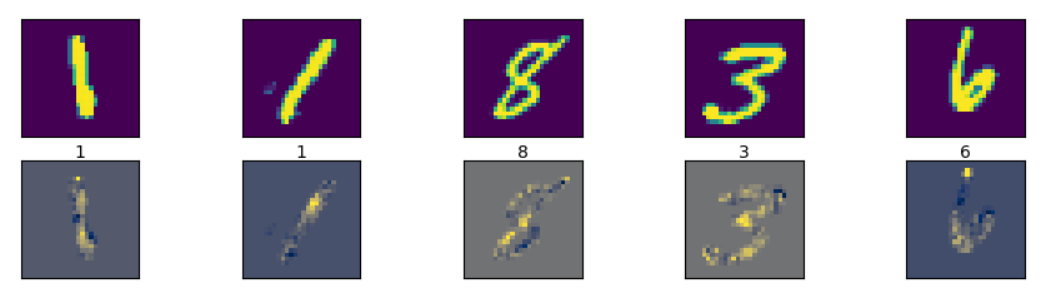
\includegraphics[width=0.6\textwidth]{grafiken/mnist_erg_1.png}
\end{figure}
}


\frame{\frametitle{Vergleich LRP $\leftrightarrow$ Heatmap}
\begin{itemize}
\item Ersetze den Wert der Neuronen $x_i$ durch den Mittelwert der Schicht.
\item Versuche, allgemeine Aussagen zu treffen.
\item Am Beispiel des MNIST Datensatz:
\item <Screenshot machen und hinzu>
\end{itemize}
%\vspace*{1cm}


}


\section{Einf\"uhrung - Convolutional Neural Networks} 
\frame{\frametitle{Dense Layer $\Leftrightarrow$ Convolutional Layer}
\begin{itemize}
\item 
\end{itemize}
}
\frame{\frametitle{Erweiterung: Mehrere Filter}
\begin{itemize}
\item Grafik
\item
\end{itemize}
}

\section{Implementierung eines Netzes zur Bilderkennung}

\frame{\frametitle{Bilderkennung mittels CNNs - Implementierung}
\begin{itemize}
\item <Abschnitt zum Beschreiben der Implementierung von CNNs>
\item Herausforderungen bei der Implementierung

\end{itemize}
}
\section{Implementierung LRP f\"ur CNNs}
\frame{\frametitle{Bilderkennung mittels CNNs - Implementierung}
\begin{itemize}
\item Theo Abschnitt zur Implementierung
\item Ergebnisse direkt dazu?

\end{itemize}
}

\section{Konzept - Deep Taylor Decomposition} 
\frame{\frametitle{Taylor Decomposition f\"ur Neuronale Netze}
\begin{itemize}
\item Problem bei der LRP bisher: Die Formeln machen Sinn und funktionieren, aber die theoretische Fundierung fehlt.
\item Mit theoretischer Fundierung sind evlt. allgemeinere Aussagen möglich.
\item Betrachte hierzu ein NN als Funktion $f: \rn^{p} \rightarrow \rn$, wobei $p$ die Inputgr\"osse bezeichnet. 
\item Nehme an, dass $f(x)> 0$ Evidenz f\"ur das gesuchte Objekt bedeutet.
\item Intuition: Verschiebe den Input, sodass $f(x)=0$. Dimensionen, in die "{}weiter"{} verschoben wurde, haben offensichtlich mehr zur Klassifizierung beigetragen.
\end{itemize}
}
\frame{\frametitle{Taylor Decomposition}
\begin{itemize}
\item Ansatz: Betrachte Taylor-Entwicklung von $f$. 
\item W\"ahle als Entwicklungspunkt $\hat{x}$ eine Nullstelle von $f$. 
\item Taylorentwicklung ist gegeben durch
\begin{align*}
f(\boldsymbol{x}) &= f(\hat{\boldsymbol{x}})+\left(\left.\frac{\partial f}{\partial \boldsymbol{x}}\right|_{\boldsymbol{x}=\hat{\boldsymbol{x}}}\right)^{\top} \cdot(\boldsymbol{x}-\hat{\boldsymbol{x}})+\varepsilon \\ 
&= 0+\sum_{p} \underbrace{\left|\frac{\partial f}{\partial x_{p}}\right|_{x=\hat{x}} \cdot\left(x_{p}-\hat{x}_{p}\right)}_{R_{p}(x)}+\varepsilon
\end{align*}
\item $R_p (x)$ stellt somit die Relevanz der $p-$ten Komponente des Inputs dar.
\item Genauigkeit h\"angt davon ab, ob Terme h\"oherer Ordnung vernachl\"assigt werden k\"onnen.
\end{itemize}
}

\frame{\frametitle{Taylor Decomposition}
\begin{itemize}
\item Problem: Wahl eines geeigneten Punkts $\hat{x}$ für das ganze Netzwerk.
\item Oft zu weit entfernt und gibt somit nicht so viele Informationen zur Entscheidungsfindung des Netzwerks.
\item Gradient Shattering (-> Montavon Vortrag, nochmal genauer nachschauen)
\item Abhilfe: Führe die Taylor Decomposition an jedem einzelnen Neuron mit einem eigenen Punkt $\hat{x}^{(j)}$ durch. 
\item Konzept der \textbf{Deep Taylor Decomposition} 
\end{itemize}
}

\frame{\frametitle{Deep Taylor Decomposition}
\begin{itemize}
\item Deep Taylor erklären
\end{itemize}
}